\documentclass[
print,
  11pt,
  table,   
  nolof,    
  nolot,
  oneside,
  final
]{fithesis3}

\usepackage[resetfonts]{cmap}
\usepackage[main=czech,english]{babel}       
%% The following section sets up the metadata of the thesis.

\thesissetup{
    university    = mu,
    faculty       = fi,
    type          = mgr,
    author        = Bc. Milan Valúšek,
    gender        =m,
    advisor       = prof. RNDr. Jiří Hřebíček\, CSc.,
    title         = {Podpora výuky matematiky v LMS Moodle s využitím Maple T.A.},
    TeXtitle      = {Podpora výuky matematiky v LMS Moodle s využitím Maple T.A.},
    keywords      = {E-learning, Learning Management system, Learning Tools Interoperability, Moodle, Maple T.A., webové služby, integrace },
    TeXkeywords   = {E-learning, Learning Management system, Learning Tools Interoperability, Moodle, Maple T.A., webové služby, integrace },
}
\thesislong{abstract}{
Práce se zabývá e-learningovými systémy LMS Moodle a Maple T.A., jejich základním stavebním prvkům a použití. Dále analyzuje možnosti rozšíření systému Moodle a existující možnosti integrace se systémem Maple T.A. V poslední části práce je navržen a implementován vlastní způsob integrace.
}
\thesislong{thanks}{
Rád bych poděkoval vedoucímu práce panu prof. RNDr. Jiřímu Hřebíčkovi, CSc. za jeho
odborné vedení práce a cenné rady a připomínky. Dále bych rád poděkoval svým rodičům a blízkým za podporu při tvorbě této práce a během celého studia. 
}
%% The following section sets up the bibliography.
\usepackage{csquotes}
\usepackage[              %% When typesetting the bibliography, the
  backend=biber,          %% `numeric` style will be used for the
  style=numeric,          %% entries and the `numeric-comp` style
  citestyle=numeric-comp, %% for the references to the entries. The
  sorting=none,           %% entries will be sorted in cite order.
  sortlocale=auto         %% For more unformation about the available
]{biblatex}               %% `style`s and `citestyles`, see:
%% <http://mirrors.ctan.org/macros/latex/contrib/biblatex/doc/biblatex.pdf>.
\addbibresource{my_bib.bib} %% The bibliograpic database within
                          %% the file `example.bib` will be used.
\usepackage{makeidx}      %% The `makeidx` package contains
              %% helper commands for index typesetting.
%% These additional packages are used within the document:
\usepackage{paralist}
\usepackage{amsmath}
\usepackage{amsthm}
\usepackage{amsfonts}
\usepackage{url}
\usepackage{menukeys}
\makeatletter\thesis@load
  \makeatletter
    \def\thesis@blocks@thanks{%
      \ifx\thesis@thanks\undefined\else
	\thesis@blocks@clear
	\begin{alwayssingle}%
	  \chapter*{\thesis@@{thanksTitle}}%
	  \thesis@thanks
	\end{alwayssingle}%
      \fi}
  \makeatother
\begin{document}


\chapter{Úvod}


Moderní svět je již v dnešní době závislý na moderních technologiích. Vyžaduje to stále více společnost, ve které technologie nevyužívají jen mladí a techničtí lidé, ale i méně technicky gramotní uživatelé. Skladba těchto uživatelů navíc je, především díky dostupnosti a rozšířenosti mobilních zařízení, velice rozmanitá a rozdíly v úrovni vzdělání, věku a rozdíly v kultuře ani sociálně-ekonomický aspekt již nehrají takovou roli \cite{itustats}. S takto rozšiřující se základnou uživatelů moderních technologií roste poptávka po nových nástrojích a pokrytí existujících služeb mobilními (online) technologiemi, které neomezují uživatele místem, časem ani způsobem konzumace.


Mezi základní služby, které tento trend následují a jdou naproti svým uživatelům, se řadí i elektronické vzdělávání, tzv. e-learning. Nicméně osobní kontakt s vyučujícím a kolektivem studentů u prezenčního studia zůstává stále důležitým aspektem v procesu vzdělávání, proto v nejbližších desetiletích e-learning klasické vzdělávání nejspíše nenahradí \cite{techvsteach}. I přesto si distanční forma studia získala důležitou pozici právě díky výhodám, které přinášejí moderní online technologie, jež dokáží odbourat řadu překážek (distance, čas, produktivita atd.). S e-learningem se také zvýšila dostupnost vzdělání pro poměrně velkou část populace, která nemůže studovat prezenčně a u nichž je individuální časový plán nutností (důchodci, zaměstnaní ad.).

Nejsou to jen nové technologie, trendy nebo systémy, jež studenty doprovázejí v distančním vzdělávání; jsou to především tutoři a materiály, které jsou prezentovány nástroji určenými pro vzdělávání. Na druhou stranu prezentace a možnosti nástroje hrají svou roli při přípravě materiálů, vzdělávání, koordinaci výuky, kooperaci a evaluaci studentů a jejich práce. Každý nástroj má své silné a slabé stránky. Jejich kombinací můžeme dosáhnout lepších výsledků, ale jen v případě, že zapojení více nástrojů ve výsledku neztíží uživateli práci. Řešením jednoduchého použití více nástrojů je jejich integrace. Právě téma integrace je zajímavé a přínosné při rozvoji e-learningu, a proto je cílem této diplomové práce integrace nástroje Maple T.A. a e-learningové platformy LMS Moodle.

V první částí diplomové práce si uvedeme definice pojmů ze světa distanční výuky. Zaměříme se blíže na LMS Moodle, který patří mezi velmi oblíbené výukové platformy, i když si s sebou nese nálepku složitého a někdy nepřehledného softwaru, a nástroj Maple T.A., který se zaměřuje na zkoušení a testování úloh především matematického zaměření. V rámci práce je vysvětleno, k čemu nástroje slouží, jak se dají použít, co nabízí a jak přistupují k uživatelům a jejich oprávněním a také jaké jsou základní stavební kameny obou systémů.

Ve druhé části práce se zaměříme na způsoby rozšíření LMS Moodle a provedeme analýzu možností integrace s nástrojem Maple T.A. Rozebereme existující konektory a podíváme se na návrh vlastního jednoduchého řešení a detaily ze samotné implementace konektoru. Rozebereme také další možnosti rozvoje navrhovaného řešení.


\chapter{Definice pojmů}
	\section{E-learning}
E-learning se rozvíjí a mění stejně rychle jako informační technologie, které využívá, a reaguje na aktuální dění ve společnosti. Proto není divu, že se nabízí více definic pojmu e-learning. Dostatečně je pojem e-learning popsán následujícími definicemi:

\begin{enumerate}
  \item „Význam slovního spojení e-learning může být brán jako elektronické vzdělávání. Elektronické vzdělávání znamená z hlediska učitele realizovat edukační proces elektronickými prostředky, v současnosti přesněji informačně-komunikačními prostředky. Elektronické učení z pozice žáka znamená realizovat těmito prostředky proces vlastního učení.“ \cite{ockajova}
  \item „E-learning je výuka s využitím výpočetní techniky a internetu.“ \cite{korviny}
  \item „E-learning zahrnuje jak teorii a výzkum, tak i jakýkoliv vzdělávací proces (s různým stupněm intencionality), v němž jsou v souladu s etickými principy používány informační a komunikační technologie pracující s daty v elektronické podobě. Způsob využívání prostředků ICT a dostupnost učebních materiálů jsou závislé především na vzdělávacích cílech a obsahu, charakteru vzdělávacího prostředí, potřebách a možnostech všech aktérů vzdělávacího procesu.” \cite{zounek}

\end{enumerate}


Nad rámec těchto definic můžeme e-learning také chápat jako samostudium prostřednictvím počítače, mobilu či jiného zařízení připojeného k internetu. Materiály u této formy výuky jsou zpravidla znovupoužitelné a jednoduše upravitelné. Nabízí učiteli téměř neomezené možnosti úprav a přístup odkudkoliv, kde má připojení k internetu. Studentům na druhé straně nabízí často okamžitou odezvu (nejedná-li se o úlohy vyžadující ruční úpravu) a dostupnost ke studijním materiálům. Nad rámec standardních služeb nabízí také nové komunikační možnosti jako fórum, skupinový chat apod.


Na druhou stranu je potřebné podotknout, že e-learning nepřináší jen výhody. Hlavní problém, který při e-learningu nastává, je absence osobního kontaktu studenta s učitelem a ostatními studenty, jelikož nedochází k rozvoji dalších dovedností, jakými jsou například sebeprezentace a schopnost vyjadřovat se. Komunikace mezi učitelem a studentem navíc postrádá bezprostřední odezvu a částečně ztrácí efektivitu při řešení problému. Vedle toho přináší zvýšené nároky na učitele a jeho přípravu materiálů. Ty musí být patřičné kvality, protože podkladové materiály musí být jasné, samo-vysvětlující a zároveň by neměly být příliš obsáhlé, aby studenta nesváděly jen k rychlé povrchní prohlídce.

Slovo e-learning se často nesprávně zaměňuje s pojmem „on-line výuka“. Vysvětleme si tedy rozdíl mezi těmito dvěma výrazy. On-line výuka předpokládá on-line (přímé) spojení mezi učitelem a studentem. Učitel tedy musí být připojený ve stejnou chvíli jako student, aby mohl komunikovat se studentem, odpovídat na jeho dotazy, radit mu, zkoušet ho. Učitel sice může být vzdálen od studenta několik desítek kilometrů, ale musí být fyzicky přítomen u počítače a interaktivně se studentem pracovat. [8] Pojem „e-learning“ kromě on-line výuky zahrnuje způsob vyučování, které rovněž probíhá vzdáleně, ale nemusí existovat přímé spojení mezi vyučujícím a studentem. Není po nich vyžadována přítomnost na stejném místě, ani ve stejný čas.


	\section{Distanční vzdělávání}

Výše zmíněné definice e-learningu mají společného jmenovatele, kterým jsou informační technologie. E-learning se tak stává prostředkem tzv. distančního vzdělávání. V následujícím textu jsou popsány základní definice distančního vzdělávání: 

      \begin{itemize}
	\item „Distanční vzdělávání je multimediální forma řízeného samostatného studia, které je koordinováno vzdělávací institucí a v němž jsou vyučující resp. konzultanti (tutoři) v průběhu vzdělávání trvale nebo převážně fyzicky odděleni od vzdělávaných. Multimediálnost zde znamená využití všech dostupných a účelných didaktických prvků a technických prostředků, kterými lze prezentovat učivo, komunikovat se studujícími, provádět průběžné hodnocení studijních pokroků a případně také hodnotit závěrečné výsledky studia. Aktuální a efektivní technologickou podporou distančního studia je metoda e-learning.“ \cite{zlamalova} 
	\item Dle \cite{prucha} se „jedná o formu studia zprostředkovaného médii (telefon, rozhlas, televize, počítač, zvl. internet a elektronická pošta aj.). Je založeno na samostatném studiu účastníků, řízeném specializovanou institucí, bez prezenčního kontaktu studujících s vyučujícími. Výuku účastníků zajišťují speciálně připravené učební materiály (výukové balíky) a jiné metody studijní podpory a hodnocení, umožňující individuální přístup.“ 
     \end{itemize}

Distančním vzděláváním se, nejen na základě zmíněných definic, myslí alternativní styl výuky, který nevyžaduje přímý kontakt mezi aktéry výuky. Naopak probíhá převážně formou samostudia, které je řízeno připravenými materiály, s případnou pomocí tutora. Využívá různých komunikačních kanálů, se zvláštním zaměřením na internet a služby s ním spojené (elektronická pošta, konference, video kanály, webové prezentace, e-learningové platformy apod.).


	\section{Learning management system}
Learning management system (zkráceně LMS) je označení jakéhokoliv balíku softwarových nástrojů sloužícího k e-learningu, které jsou dostupné online, nejčastěji z webového rozhraní. Hlavním, nikoliv jediným, nástrojem je tvorba, distribuce a administrace vzdělávacích kurzů a materiálů. Vedle nástroje pro správu kurzů LMS obsahuje také tyto části \cite{lms}:
\begin{itemize}
	\item Evidence a správa žáků
	\item Katalog výukových kurzů a objektů
	\item Správa studijních plánů
	\item Evidence hodnocení žáků
	\item Testování a zkoušení žáků
	\item Správa přístupových práv
	\item Komunikační nástroje
	\item Autorské nástroje k vytváření výukových kurzů a objektů
	\item Úložiště výukového obsahu
\end{itemize}
Jednotlivá řešení LMS nemusí nutně zahrnovat všechny tyto nástroje a naopak mohou nabízet širší paletu nástrojů.

	\section{Learning Tools Interoperability}
Learning Tools Interoperability (LTI) je specifikace vytvořená organizací IMS Global Learning Consortium a jejím cílem je ustanovení standardního přístupu k integraci výukových aplikací (často poskytované jako služby třetích stran) s výukovými platformami, jakými jsou LMS, CMS, portály, výukové repozitáře a další prostředí pro podporu výuky. V praxi to znamená přímočarou a bezimplementační integraci nástrojů s odlišnou funkcionalitou pomocí jednotného rozhraní, což vede ke snížení časových i finančních nákladů při integraci napříč systémy. \cite{imslti}

Klíčovým konceptem LTI je „konzument” a „poskytovatel”. Specifikace udává jednotné rozhraní mezi e-learningovým nástrojem poskytujícím služby a e-learningovou platformou konzumující služby. V praxi je typických konzumentem LMS na bázi Moodlu nebo Blackboardu, ale není to podmínkou, a typickým poskytovatelem je software třetích stran podobný nástrojům Wimba, Mahara e-portfolio nebo třeba Maple T.A.. Specifikace LTI podporuje širší definici konzumenta i poskytovatele zahrnující například studentské portály (konzumenti) a různorodé externě hostované funkcionality (poskytovatelé). \cite{imsltiinvest}


Specifikace LTI má dvě hlavní větve: LTI 1 a LTI 2, kterými lze integrovat systémy. LTI 1 bylo poprvé uvolněno v roce 2006, kdy bylo příliš komplexní a neujalo se. Další vydání se snažila specifikaci zjednodušit. V roce 2012 je vydána verze LTI 1.1 a později téhož roku LTI 1.1.1. Právě tyto verze se využívají pro integraci mezi systémy, poskytují základní a jednoduché rozhraní pro komunikaci a přenos informací.

LTI 2 byla dlouho vyvíjená verze, která byla vydána v lednu roku 2015. Umožňuje přenášení více informací (aktivní přenos výsledků, více sofistikovaný přenos informací a rozšiřitelnou množinu informací pro hlubší integraci) mezi systémy v obou směrech komunikace a přináší větší kontrolu a svobodu v umístění odkazů na poskytující software. Vzhledem k tomu, že se jedná o relativně novou specifikaci, není její implementace tolik rozšířená. \cite{imslti20}



\chapter{LMS Moodle}
Cílem této kapitoly je představit LMS Moodle, jeho základní stavební kameny, práci s kontexty, uživatelskými rolemi  a postup založení a nastavení konkrétního kurzu.
	\section{Co je to Moodle?}
Moodle je software pro tvorbu výukových systémů a elektronických kurzů na internetu. Jedná se o neustále se vyvíjející projekt (již od roku 1999), navržený na základě sociálně konstruktivistického\footnote{Více na https://docs.moodle.org/archive/cs/V\%C3\%BDchodiska.}  přístupu ke vzdělávání \cite{moodle-what-is}.  Slovo Moodle vychází z akronymu pro Modular Object-Oriented Dynamic Learning Environment (Modulární objektově orientované dynamické prostředí pro výuku). A s čím tedy Moodle přichází?
		\begin{figure}
		  \begin{center}
		    
\includegraphics[width=60mm]{images/moodle-logo.png}
		   \end{center}
		  \caption{Oficiální logo Moodlu. \cite{moodle-logo}}
		  \label{fig:moodlelogo}
		\end{figure}

	\section{Historie}
		\begin{figure}
		  \begin{center}
		    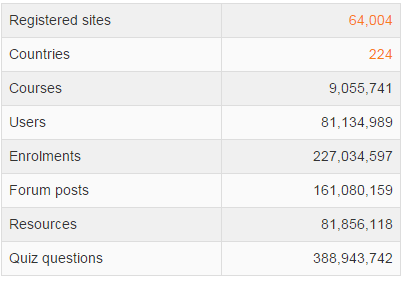
\includegraphics[width=80mm]{images/statistiky-moodle.png}
		   \end{center}
		  \caption{Počet kurzů a uživatelů ze stránek registrovaných na Moodle.org.   \cite{moodle-stats}}
		  \label{fig:moodlestats}
		\end{figure}

	\section{Vlastnosti Moodlu}

		\subsection{Licence}
		\subsection{Prerekvizity}
		\subsection{Rozvoj}
		\subsection{Výhody a nevýhody}
	\section{Kurz}
		\subsection{Rozložení}
		\subsection{Výukové moduly}
		\subsection{Bloky}
	\section{Uživatelské role a kontext}

		\begin{figure}
		  \begin{center}
		    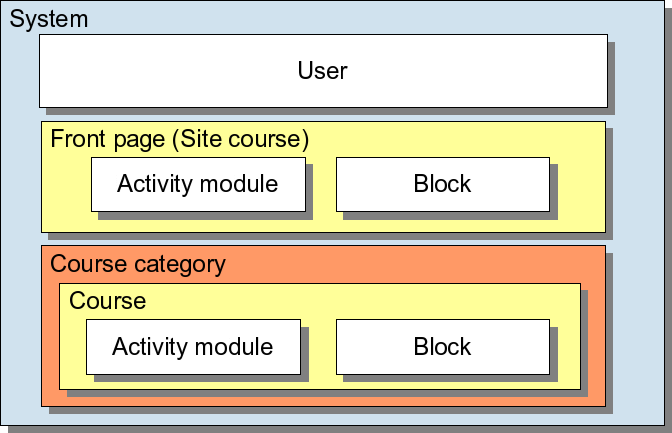
\includegraphics[width=100mm]{images/moodle-context.png}
		   \end{center}
		  \caption{Grafické zobrazení hierarchie kontextů.   \cite{moodle-context}}
		  \label{fig:moodlecontext}
		\end{figure}

	\section{Vytvoření kurzu a jeho nastaven}

		\begin{figure}
		  \begin{center}
		    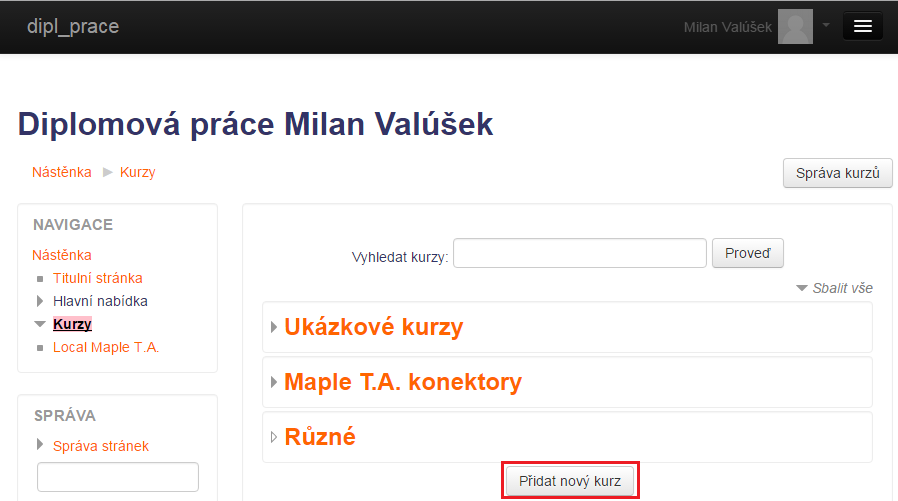
\includegraphics[width=120mm]{images/kurzy-pridani.png}
		   \end{center}
		  \caption{Náhled obrazovky s kategoriemi kurzy (uživatel s právy vytvořit kurz).  }
		  \label{fig:moodlekurzypridani}
		\end{figure}

		\begin{figure}
		  \begin{center}
		    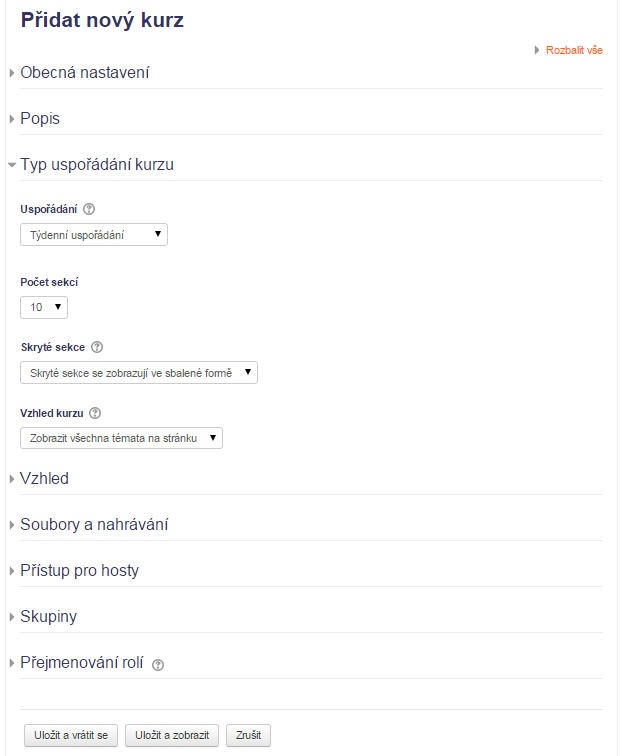
\includegraphics[width=120mm]{images/kurzy-pridani-detail.png}
		   \end{center}
		  \caption{Náhled na formulář pro přidání kurzu.}
		  \label{fig:moodlekurzypridanidetail}
		\end{figure}

\chapter{Maple T.A.}
	\section{Co je to Maple T.A.?}
		\begin{figure}
		  \begin{center}
		    
\includegraphics[width=60mm]{images/MapleTA_logo.jpg}
		   \end{center}
		  \caption{Oficiální logo Maple T.A.  \cite{maple-logo}}
		  \label{fig:maplelogo}
		\end{figure}

	\section{Licencování}
	\section{Předpoklady pro instalaci}
	\section{Základy aplikace}
		\subsection{Otázka (Question)}

		\begin{figure}
		  \begin{center}
		    
\includegraphics[width=60mm]{images/MapleTA_logo.jpg}
		   \end{center}
		  \caption{Oficiální logo Maple T.A.  \cite{maple-logo}}
		  \label{fig:maplelogo}
		\end{figure}

		\begin{figure}
		  \begin{center}
		    
\includegraphics[width=60mm]{images/MapleTA_logo.jpg}
		   \end{center}
		  \caption{Oficiální logo Maple T.A.  \cite{maple-logo}}
		  \label{fig:maplelogo}
		\end{figure}

		\begin{figure}
		  \begin{center}
		    
\includegraphics[width=60mm]{images/MapleTA_logo.jpg}
		   \end{center}
		  \caption{Oficiální logo Maple T.A.  \cite{maple-logo}}
		  \label{fig:maplelogo}
		\end{figure}

		\begin{figure}
		  \begin{center}
		    
\includegraphics[width=60mm]{images/MapleTA_logo.jpg}
		   \end{center}
		  \caption{Oficiální logo Maple T.A.  \cite{maple-logo}}
		  \label{fig:maplelogo}
		\end{figure}

		\subsection{Úkol (Assignment)}
		\subsection{Kniha hodnocení (Gradebook)}
	\section{Uživatelské role}
	\section{Vytvoření úkolu}
\chapter{Analýza}
	\section{Struktura zdrojových kódů Moodlu}
	\section{Analýza konektorů od Maple T.A.}
		\subsection{Klasický konektor}
		\subsection{LTI konektor}

\chapter{Implementace}
	\section{Webové služby Maple T.A.}
		\subsection{Kontrola připojení}
		\subsection{Vytvoření a ukončení relace}
		\subsection{Získávání a manipulace s daty}
		\subsection{Maple T.A. Launcher služby}
		\subsection{Grade pushing}
		\subsection{Monitoring}
	\section{Návrh a porovnání s ostatními konektory}
	\section{Databázový model}
	\section{Struktura modulu a její realizace}

		\begin{figure}
		  \begin{center}
		    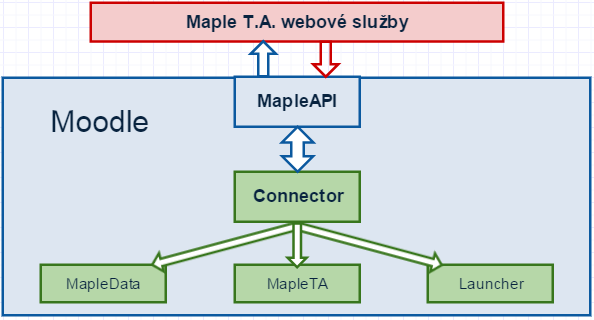
\includegraphics[width=100mm]{images/struktura_modulu.png}
		   \end{center}
		  \caption{Struktura navrhovaného modulu}
		  \label{fig:strukturamodulu}
		\end{figure}

		\begin{figure}
		  \begin{center}
		    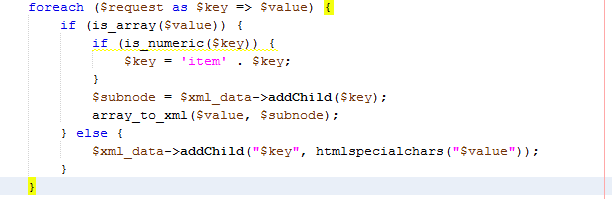
\includegraphics[width=100mm]{images/prevod_na_xml.png}
		   \end{center}
		  \caption{Algoritmus k převedí asociativního pole na XML}
		  \label{fig:prevodnaxml}
		\end{figure}

		\begin{figure}
		  \begin{center}
		    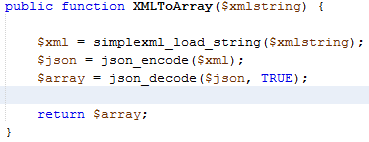
\includegraphics[width=100mm]{images/xml_na_pole.png}
		   \end{center}
		  \caption{Webové služby vrací data v podobě XML, tímto voláním se převedou na asociativní pole.}
		  \label{fig:prevodnapole}
		\end{figure}

		

	\section{Detaily implementace}
		\subsection{Vytovření nové instance}
		\begin{figure}
		  \begin{center}
		    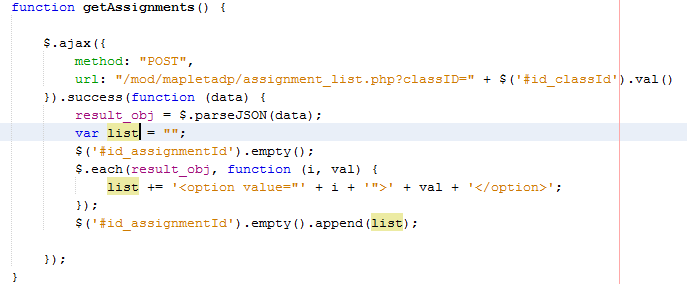
\includegraphics[width=100mm]{images/ajax-volani.png}
		   \end{center}
		  \caption{Voláním PHP za pomoci AJAXu se získávají hodnoty pro závislé pole formuláře.}
		  \label{fig:volaniajax}
		\end{figure}


		\subsection{Nová naplánovaná úloha}

		\begin{figure}
		  \begin{center}
		    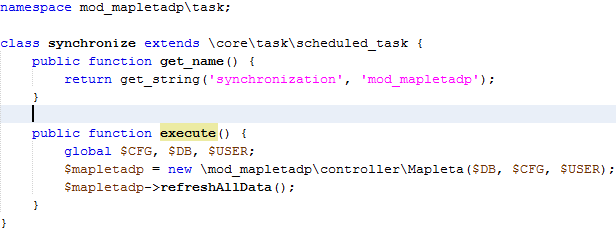
\includegraphics[width=100mm]{images/cron-trida.png}
		   \end{center}
		  \caption{Implementace třídy je využíta jako naplánovaná úloha. }
		  \label{fig:crontrida}
		\end{figure}

		\begin{figure}
		  \begin{center}
		    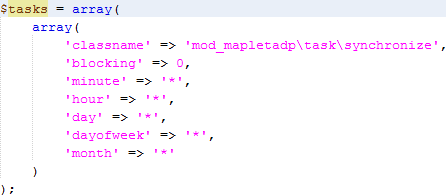
\includegraphics[width=100mm]{images/cron-registrace.png}
		   \end{center}
		  \caption{Ukázka záznamu z pole, které Moodle využivá při instalaci nové naplánované úlohy.}
		  \label{fig:cronregistrace}
		\end{figure}
\chapter{Diskuze}

\chapter{Závěr}




\printbibliography[heading=bibintoc]
\listoffigures
\listoftables




\makeatletter\thesis@blocks@clear\makeatother
\phantomsection %% Print the index and insert it into the
\addcontentsline{toc}{chapter}{\indexname} %% table of contents.

\makeatletter\thesis@blocks@clear\makeatother

\renewcommand{\theHchapter}{A\arabic{chapter}}
\appendix %% and start the appendices.

\chapter{An appendix}
Here you can insert the appendices of your thesis.

\end{document}
